\documentclass[docid=PA07]{tcom_PA}
\begin{document}
\setcounter{chapter}{6}
\exam{Preparation Activity 7 - Context-Free Grammars (CFGs)}
{
\renewcommand{\thesubsubsection}{\thesubsection\alph{subsubsection}}
\newcommand{\lmd}{\xRightarrow[lm]{}}
\question{Exercise 1}
\questionitem{Item a}
\begin{definition}[CFG ambiguity]
A CFG is \textit{ambiguous} iff there exists a string $w$ that has at least two different syntax trees.
\end{definition}
This CFG is ambiguous, because the string $a+a \times a$ has two different syntax trees:
\begin{center}
\begin{minipage}{0.4\linewidth}
	\begin{center}
		\begin{tikzpicture}
			\Tree 	[.$E$
						[.$E$
							[.$I$
								$a$
							]
						]
						$+$
						[.$E$
							[.$E$
								[.$I$
									$a$
								]
							]
							$\times$
							[.$E$
								[.$I$
									$a$
								]
							]
						]
					]
	  	\end{tikzpicture}
	\end{center}
\end{minipage}
\begin{minipage}{0.4\linewidth}
	\begin{center}
		\begin{tikzpicture}
			\Tree 	[.$E$
						[.$E$
							[.$E$
								[.$I$
									$a$
								]
							]
							$+$
							[.$E$
								[.$I$
									$a$
								]
							]
						]
						$\times$
						[.$E$
							[.$I$
								$a$
							]
						]
					]
	  	\end{tikzpicture}
	\end{center}
\end{minipage}
\end{center}
\questionitem{Item b}
\begin{alignat*}{6}
	E
	& \lmd (E)
	&&\lmd (E+E)
	&&\lmd ((E)+E)
	&&\lmd ((I)+E) \\
	& \lmd ((a)+E)
	&&\lmd ((a)+(E)) 
	&&\lmd ((a)+(E \times E))
	&&\lmd ((a)+(I \times E)) \\ 
	& \lmd ((a)+(a \times E)) 
	&&\lmd ((a)+(a \times I)) 
	&&\lmd ((a)+(a \times b)) 
\end{alignat*}
\begin{center}
	\begin{tikzpicture}
		\Tree 	[.$E$
					$($
					[.$E$
						[.$E$
							$($
							[.$E$
								[.$I$
									$a$
								]
							]
							$)$
						]
						$+$
						[.$E$
							$($
							[.$E$
								[.$E$
									[.$I$
										$a$
									]
								]
								$\times$
								[.$E$
									[.$I$
										$b$
									]
								]
							]
							$)$
						]
					]
					$)$
				]
	  \end{tikzpicture}
\end{center}
\question{Exercise 2}
\questionitem{Item a}
G2 is not ambiguous. It however does not represent the same language of G1, something we can prove by considering the string $a \times (a+a)$, which by G1 has a derivation
\begin{alignat*}{6}
	E
	&\lmd E \times E
	&&\lmd I \times E
	&&\lmd a \times E
	&&\lmd a \times (E)
	&&\lmd a \times (E+E) \\
	&\lmd a \times (I+E)
	&&\lmd a \times (a+E)
	&&\lmd a \times (a+I)
	&&\lmd a \times (a+a)
\end{alignat*}
but does not have a derivation by G2, since an expression $E$ can only be extended to the left as an expression, and not to the right.
\questionitem{Item b}
G3 is not ambiguous. It however does not represent the same language of G1, something we can prove by considering the string $a \times a+a$, which by G1 has a derivation
\begin{alignat*}{6}
	E
	&\lmd E \times E
	&&\lmd I \times E
	&&\lmd a \times E
	&&\lmd a \times E+E \\
	&\lmd a \times I+E
	&&\lmd a \times a+E
	&&\lmd a \times a+I
	&&\lmd a \times a+a
\end{alignat*}
\questionitem{Item c}
The problem is that G4 describes the string $(a)a$ through the derivation
\begin{alignat*}{7}
	E
	&\lmd J
	&&\lmd I
	&&\lmd Ia
	&&\lmd (E)a
	&&\lmd (J)a
	&&\lmd (I)a
	&&\lmd (a)a
\end{alignat*}
and G1 can not describe this string.
\questionitem{Item d}
G5 achieves non-ambiguity because it uses new variables to distinguish levels of priority and association rules. Thus, an expression $E$ can only be decomposed into one or a sum of several terms $T$, where each term $T$ can only be decomposed into an identifier $I$, or be promoted again to expression but only if inside parenthesis $(E)$.
}
\end{document}
